\documentclass[10pt,a4paper]{article}
\usepackage[T1]{fontenc}
\usepackage[utf8]{inputenc}
\usepackage{newtxtext,newtxmath}
\usepackage[a4paper,textwidth=150mm,textheight=235mm,centering,headheight=13pt]{geometry}
\usepackage{microtype,amsmath,booktabs,tabularx,array,longtable,graphicx}
\usepackage[numbers,sort&compress]{natbib}
\usepackage[english]{babel}
\usepackage{xurl}
\usepackage{fancyvrb,flafter,needspace,placeins}
\usepackage[hidelinks]{hyperref}
\usepackage{fancyhdr,titlesec}
\titleformat{\section}{\large\bfseries}{\thesection.}{.5em}{}
\titleformat{\subsection}{\normalsize\bfseries}{\thesubsection}{.5em}{}
\setlength{\parskip}{4pt}\setlength{\parindent}{0pt}
\setlength{\emergencystretch}{3em}\setlength{\tabcolsep}{4pt}
\renewcommand{\arraystretch}{1.15}\renewcommand{\bibfont}{\footnotesize}
\renewcommand{\thesection}{S\arabic{section}}
\setcounter{secnumdepth}{2}
\pagestyle{fancy}\fancyhf{}\fancyhead[L]{\small HealthGraphBench | RC2 working revision}
\fancyhead[R]{\small Scientific supplement}\fancyfoot[C]{\small\thepage}
\renewcommand{\headrulewidth}{0pt}\raggedbottom
\clubpenalty=10000\widowpenalty=10000
\newcommand{\src}[1]{{\small\nolinkurl{#1}}}
\hypersetup{pdftitle={HealthGraphBench RC2 — Scientific supplement},pdfauthor={},pdfsubject={Working manuscript revision; author approval and submission remain outstanding}}
\begin{document}

\begin{center}
{\small SCIENTIFIC SUPPLEMENT • RC2 WORKING REVISION • NOT AUTHOR-APPROVED}\par\vspace{7pt}
{\LARGE\bfseries HealthGraphBench — RC2}\par\vspace{6pt}
{\large Methods, provenance, and supplementary analyses}
\end{center}

\textbf{Inherited R5 evidence.} The R5 delivery retains health-data results, both R2 bootstraps, and additions verified in R4: CMS AP and decile boundaries, recoverable MAUDE candidate distributions, three real compacts, and their replays. The GraphSAGE core was compared with the complete source file and rerun on a synthetic instance. Network acquisition of frozen outputs succeeded. R5 adds the audit at the package root and harmonizes presentation, without a new experiment. Omissions in the inherited MAUDE summary are distinguished from current results in S3 and S10.

\textbf{Historical R6 collection.} The R6 B1/B2 collection reacquired nine official MAUDE archives and reproduced historical ingestion and example preparation without model training or new scores. These statements describe that historical collection only; separate health-model training for RC2 analyses C and D1 is reported in S11.

\section{Evidence scope and package inventory}
\label{supp:evidence}
Commit \nolinkurl{b010d5a49eae56837a920b2e30dece41c42c0c44} identifies the benchmark source state\cite{hgb2026,hgbresults}. DOI \nolinkurl{10.5281/zenodo.22796551} identifies v0.2: its resolution and the public Zenodo record were checked online in R4. This DOI does not identify the manuscript package. Completion changes neither frozen experimental artifacts nor a remote repository.

\begin{tabularx}{\linewidth}{@{}p{31mm}Xp{39mm}@{}}
\toprule
Evidence & Use in the study & Verification level\\
\midrule
Task definitions, v0.1/v0.2 reports, and unified summary & Targets, periods, results, and existing intervals & Targeted reading documented in R2; transcriptions retained in R3\\
v0.1 analysis & Annual AUC/AP/Brier, counts, and history depth & Compact-summary values; top-decile P/R extracted separately in R2 from frozen predictions\\
Code for the three tasks & Heuristics, conventions, training constants, and ties & Targeted R2 reading, not an exhaustive audit; description retained\\
Project history and ClinicalTrials memo & Task selection and reasons for deferral & Available records, not a complete log of human decisions\\
Individual MAUDE files, Part D rankings, and CMS predictions & Inputs for complementary analyses & Fingerprints rechecked, network downloads and three real replays executed in R4\\
Synthetic-control code & Scope of direct-score AUC & Reread at pinned commit for R3; not executed\\
Raw FDA/CMS archives & Ingestion and historical reconstruction & Nine official MAUDE archives ingested for B1/B2; CMS and comprehensive FDA/CMS reconstruction remain outside scope\\
\bottomrule
\end{tabularx}

\textbf{Versions and evidence.} R2 added available descriptors, the CMS decomposition, the differences plot, the two bootstraps, and annual deciles. R3 preserves numerical files byte-for-byte and corrects the synthetic-control scope, provenance declarations, and printed commands. Historical status is in \src{history/R3/data/revision_status_R3.json}; inherited declarations are archived under \src{history/R2}. \src{data/source_map_R3.csv} distinguishes reread sources from supplied files. Analyses and external fingerprints documented in R2 are not presented as independently reproduced in R3.

\textbf{R4 evidence retained through R5; historical R6 collection.} AP identities and reconstructed CMS counts remain summary-based checks. Exact calculations, candidate distributions, and real compacts are separated under \src{data/real_R4}. The R4 synthetic GraphSAGE-core diagnostic used a synthetic instance only; this does not describe the separate RC2 health-model training in S11. Historical R5 statuses are in \src{data/revision_status_R5.json}; the R6 MAUDE tables and prepared snapshots are under \src{data/real_R6/maude_B}, with acquisition and replay evidence in \src{verification/real_R6}. Those historical records are neither checkpoint inspection nor recovered optimizer logs. R5 delivery checks remain under \src{verification/r5}; historical artifact names are unchanged.

\textbf{Contents and versions.} The earlier RC1 delivery comprised five PDFs and their LaTeX sources in \src{HealthGraphBench_FAIA_LaTeX_RC1.zip}. This is a historical archive, not the RC2 working package. RC2 retains the historical results and adds the evidence described in S11. The inherited \src{SHA256SUMS} records the prior package, not the current RC2 working copy or external inputs. The prior inventory is in \src{README_EN.md}.

\par\Needspace{8\baselineskip}
\section{Method definitions and retained configurations}
\label{supp:methods}
\subsection{Historical MAUDE: histories, heuristics, and training}
For product $p$, $H_p$ is the set of prior problems and $U_c$ the set of products historically associated with problem $c$. The peer set is $N_p=(\bigcup_{d\in H_p}U_d)\setminus\{p\}$. Neighbor frequency is $|N_p\cap U_c|$; global popularity is $|U_c|$. Each distinct peer contributes once, regardless of report volume or the number of shared problems. The MAUDE heuristic has neither Jaccard weighting nor degree normalization. Missing support gives zero. Candidates are all previously known problems outside $H_p$; ties are resolved by descending score, descending global support, then ascending code\cite{hgbcode}.

The twelve tabular variables are: $\log(1+x)$ of prior product and problem reports, the number of products associated with the problem, the number of neighbors associated with it, and the number of products associated with it during the four most recent quarters; the problem's recent-support fraction; $\log(1+x)$ of product manufacturers and their products' cumulative activity; product and problem ages in quarters; $\log(1+x)$ of parent-problem prevalence; and the product's recent-report fraction. They therefore already include relational information: “tabular” does not mean “strictly local.”

The tabular path accumulates first eligible links and one deterministic historical non-positive per positive, with features built before the target quarter is added. Refits at 2023Q1, 2024Q1, and 2025Q1 use only rows already accumulated. Embedding methods fit their representations on the historical graph available at those refits, not on the same first-occurrence table. This difference in objectives and examples means their performance gap cannot be attributed to aggregation alone.

\begin{tabularx}{\linewidth}{@{}p{36mm}X@{}}
\toprule
Method & Frozen-path constants and qualification\\
\midrule
MAUDE logistic & 40 epochs; learning rate 0.15; $L_2=0.01$; standardization on training rows.\\
Boosted stumps & One-level trees; 12 rounds; learning rate 0.08.\\
Spectral factorization & Rank 8; 18 iterations.\\
BPR + fixed one-hop averaging & Dimension 8; 4 epochs; post-training combination of 0.5 target vector and 0.5 mean neighbor vector. No end-to-end learned message passing.\\
Historical one-hop GraphSAGE (v0.1) & Dimension 8; 3 epochs; 8 neighbors; learning rate 0.02; regularization 0.0005; BPR loss; $\tanh$ activation; trainable node inputs and shared transforms.\\
\bottomrule
\end{tabularx}

GraphSAGE samples neighbors; negative examples are determined by hashes, with no runtime random-number generator according to repository metadata. This makes the execution reproducible, not stable under changes to the choices.

Inductive generalization to nodes absent from the latest refit is not evaluated separately. These cases receive the zero fallback score; their frequency among evaluated observations is documented in S10. BPR triplets depend on the historical graph at refit. Using the same loss function does not make these examples comparable to tabular rows.

Tabular counts at the three historical refits, graph inventories, and triplet/step counts implied by the frozen loops are reconstructed from raw archives and prepared histories; details are in S10. For this historical collection, BPR/GraphSAGE step totals are implications of frozen code, not observed optimizer logs, and checkpoints/vectors were not inspected. The original collection added no aggregation ablation; the distinct RC2 D1 comparison is reported in S11. The separate extracted-core diagnostic remains described in S8\cite{hgbcode,hgbresults,hamilton2017}.

\subsection{CMS: two logistic regressions, not a GNN--tabular contest}
The models use eleven local numeric features and state indicators: prior inspection and serious-deficiency counts, their prior rate, inspection and deficiency counts in 365- and 730-day windows, time since the previous inspection, facility age, and prior and 365-day owner-change counts. Counts use $\log(1+x)$; time is capped at 1,460 days and divided by 365.25; age is capped at 100 years. Rates are not logged.

The augmented model adds twelve features: counts of owners, peers, and peers with history; peer prior inspections and deficiencies and their rate; peer inspections and deficiencies over 365 days and their rate; peer deficiencies over 730 days; and numbers of peers with at least one deficiency over 365 and 730 days. Counts are logged. Rates divide totals, with zero for an empty denominator; they are not unweighted means of facility rates.

CHOW identifiers \src{PAC:associate} take priority. For CCNs without a record in that representation, the code uses normalized current names, with role filters. This is a fallback, not a systematic union. Peer CCNs are deduplicated and the target is excluded. A start date on or before the target passes the filter; incomplete end dates prevent this from being treated as a complete legal history. Names do not certify legal-entity identity. Peer inspections remain strictly before the target. These limitations concern historical availability as well as entity resolution\cite{hgbcode}.

The two logistic models are standardized on training data and fitted with 300 iterations, learning rate 0.08, and $L_2=0.05$. For year $y$, rows from 2019 through $y-1$ are used. The prevalence reference is the proportion of positives in that training set; it is constant during the target year and recalculated the following year. The score is reconstructed immediately before the Health Standard inspection; the model does not predict inspection timing.

\subsection{Part D: representations and references}
Rows are mapped to the exact generic name after trimming surrounding spaces. Blank generic names are excluded; claims and specialties are aggregated at prescriber--generic--year level. This is neither RxNorm mapping nor clinical equivalence. Specialty score counts prescribers with the drug in their history and the same specialty in their latest observed year. A missing or non-unique specialty triggers fallback to global popularity.

Overlap sums Jaccard similarities between the target history and histories of peers with at least one shared drug, for peers historically associated with the candidate. Neither prescription volume nor total number of peers normalizes this sum. Ties are resolved by descending score, descending prior global support, then ascending generic key\cite{hgbcode,hgbpartd}.

Logistic regression uses ten features: global prescriber support, total and mean global claims, prescriber history size and claim volume, drug history-year count and age feature, specialty support, specialty fraction, and specialty availability. Count/age features labelled \src{log_*} are transformed in the source path. Training includes historical positive relationships and up to five historical non-links per positive; negatives are used for training only.

Logistic regression uses 18 epochs, learning rate 0.10, and $L_2=0.01$. BPR uses dimension 12, five epochs, three negatives per positive, learning rate 0.03, regularization 0.001, and specialty weight 0.35; it performs no message passing. Models are refitted before each 2023/2024 target. No exhaustive search or equalization of tuning budgets is documented.

\par\Needspace{17\baselineskip}
\subsection{Synthetic control: what is actually measured}
\label{supp:control}
The control in \src{healthgraphbench/controls/synthetic.py}, reread at the pinned commit, projects associations starting before 1 January 2024 into CCN neighborhoods. This filter does not certify a complete history of active ownership. It generates $x_i\sim\mathcal N(0,1)$ for each node, computes the mean of neighboring $x_j$, and standardizes it to $z_i$ using the subset called ``training'' (70\,\% of nodes). Labels follow
\[
Y_i\sim\mathrm{Bernoulli}\!\left(\sigma(-1+0.5x_i+\beta z_i)\right),
\qquad \sigma(a)=(1+e^{-a})^{-1}.
\]
The code directly measures the AUC of $z_i$ and of $x_i$ on test nodes. The training subset is used for standardization, not for fitting the CMS logistic regressions. At $\beta=0$, the relational signal does not enter the labels, but the local term $0.5x_i$ remains. Retained values for seeds 301, 302, and 303 are a signal-construction and measurement diagnostic; they validate neither the CMS models nor MAUDE GraphSAGE\cite{hgbcontrols}. R3 corrects this interpretation without rerunning the control.



\section{Populations and scope of documented data}
\label{supp:population}
The counts below combine frozen summaries, the R2 extraction of descriptors from individual files, and the limited R6 ingestion of raw MAUDE archives. MAUDE validation/test counts and candidate descriptors for positive-containing observations below retain their historical scope; the B1/B2 tables report training inputs and reconstructed representation coverage separately. A MAUDE observation is a product--quarter with at least one positive; a CMS observation is a target inspection; a Part D observation is an eligible prescriber--year. Resampled units do not replace these denominators.

\begin{tabularx}{\linewidth}{@{}p{35mm}rrX@{}}
\toprule
Split & Observations & Positives & Details\\
\midrule
MAUDE validation 2023 & 3,483 & 7,705 & Positive links; 1,641 distinct products\\
MAUDE test 2024--2025 & 6,370 & 13,174 & Positive links; 2,026 distinct products\\
CMS validation 2023 & 2,661 & 408 & 2,660 distinct CCNs\\
CMS test 2024 & 8,909 & 1,253 & 8,881 distinct CCNs\\
CMS test 2025 & 10,076 & 1,170 & 9,990 distinct CCNs\\
CMS pooled test & 18,985 & 2,423 & 13,889 distinct CCNs\\
Part D validation 2023 & 2,000 & 5,794 & Links; 1,035 observations with positives\\
Part D test 2024 & 2,000 & 5,476 & Links; 1,019 observations with positives\\
\bottomrule
\end{tabularx}

\textbf{Recovered Part D descriptors.} Frozen outputs also provide historical and training counts, plus candidate-list sizes for the 2023 validation and 2024 test cohorts. Candidate quantiles use linear interpolation over all 2,000 eligible prescribers in each cohort.

\begin{table}[!htbp]\centering\small
\caption{Descriptors of the Part D generic-name representation extracted from retained results.}
\begin{tabularx}{\linewidth}{@{}Xrr@{}}
\toprule
Descriptor & Validation 2023 & Test 2024\\
\midrule
Drugs in history & 1,007 & 1,042\\
Historical prescriber--drug edges & 58,472 & 60,200\\
Logistic training rows & 337,702 & 349,460\\
Positive rows & 58,472 & 60,200\\
Negative rows & 279,230 & 289,260\\
BPR parameter updates & 877,080 & 903,000\\
Specialty nodes & 71 & 72\\
Fallback to global popularity & 0/2,000 & 0/2,000\\
Candidates: minimum & 613 & 675\\
Candidates: first quartile & 974 & 1,008\\
Candidates: median & 997 & 1,032\\
Candidates: third quartile & 1,004 & 1,039\\
Candidates: maximum & 1,006 & 1,041\\
Mean number of candidates & 977.764 & 1,011.9\\
\bottomrule
\end{tabularx}
\end{table}

These descriptors are transcribed in \src{data/available_descriptors_R2.json}. Extraction verified input and source-report SHA-256 fingerprints; it did not reconstruct raw sources or rerun training.

CMS has 10,313 test observations with one prior inspection (1,341 positives), and 8,672 with at least two (1,082 positives). The report characterizes retained history as one or two inspections. These strata do not count all care or inspections ever received by facilities. Current extracts, provider selection, and a limited number of cycles truncate history\cite{hgbanalysis,hgbresults}.

\textbf{Reconstructed CMS training counts.} Let $n_0,p_0$ be the pre-2023 counts and $c_{23},c_{24}$ the recorded prevalence constants, 0.1181026137463698 and 0.13793103448275862. The annual protocol adds all 2,661 inspections and 408 positives from 2023\cite{hgbcode}. Under this protocol,
\[
 c_{23}=p_0/n_0,\quad c_{24}=(p_0+408)/(n_0+2661),\qquad
 n_0=\frac{408-2661c_{24}}{c_{24}-c_{23}}=2066.
\]
This gives $p_0=244$ and the counts below. The 2025 constant is separately recovered as $1905/13636=0.1397037254326782$. Integers and all three ratios are numerically checked by \src{summary_identities_R4.py}.
\begin{table}[!htbp]\centering\small
\caption{CMS counts reconstructed algebraically under the stated protocol, not read directly from training rows.}
\input{tables/cms_training_R4_en.tex}
\end{table}

\par\Needspace{5\baselineskip}
\textbf{Extracted MAUDE descriptors.} Running \src{extract_descriptors_R4.py} on the verified frozen file gives the distributions below for total candidate counts per distinct product--quarter with at least one positive. Quantiles use linear interpolation; sampled positive/negative rows do not weight an observation multiple times.

\begin{table}[!htbp]\centering\small
\caption{MAUDE candidates for positive-containing observations only. Zero-positive observation counts are unavailable in this export.}
\begin{tabular}{@{}lrrrrrr@{}}\toprule
Split & Observations & Min. & Q1 & Median & Q3 & Max.\\\midrule
Validation 2023 & 3,483 & 165 & 445 & 482 & 504 & 516\\
Test 2024--2025 & 6,370 & 151 & 444 & 485 & 510 & 533\\\bottomrule
\end{tabular}
\end{table}

Means are 464.710881 and 467.057457. These observations contain 7,705 and 13,174 positive links, respectively. Results and scope are in \src{data/real_R4/maude_descriptors.json}.

\textbf{Inherited descriptors and R6 scope.} The inherited R4 MAUDE export contains neither \src{training_row_counts_at_refit} nor \src{quarterly_first_edges}; its candidate descriptors concern only positive-containing product--quarters and do not cover zero-positive observations or the full candidate history. These omissions describe the earlier summary, not the current collection: raw MAUDE archives and prepared histories re-ingested in R6 provide refit counts and node/pair coverage for all twelve quarters, reported in S10. This collection remains limited to evaluated positive-containing product--quarters and all eligible candidates within them; it does not extend the population to zero-positive observations. Inventories are reconstructed, not read from checkpoints; a zero score is not used to infer a missing vector. CMS counts remain algebraically reconstructed because training rows are unavailable. Historical public availability, the human decision log, extensive ablations, and comparable resources also remain unestablished.

\section{Chronology and task selection}
\label{supp:chronology}
\begin{tabularx}{\linewidth}{@{}p{30mm}Xp{39mm}@{}}
\toprule
Record & What is established & What the record does not establish\\
\midrule
v0.1 core & MAUDE and CMS retained despite adverse or uncertain findings; definitions and executions preserved & A common criterion fixed before results were examined\\
15 September 2026 & Date carried by the v0.1 execution and analyses used & Exact date of each scientific decision or human access to test results\\
Part D extension & Bounded v0.2 cohort and task definition; previously run methods retained & Independent replication of v0.1 experiments\\
16 September 2026 & Compact Part D record and v0.2 package release; packaging commit at 13:38:48 UTC & Training date for every model; the compact adapter is not new training\\
ClinicalTrials memo & Deferral explicitly motivated by relational instability & Performance-independent exclusion\\
29 September 2026 & R2: documented analyses; R3: package corrections and checks & Reopening an unexamined test period\\
\bottomrule
\end{tabularx}

The project also documents abandoned product--label linkage directions whose predictive definition remained insufficiently defensible, and a human-evaluation direction whose independent approval was not completed. These reasons differ from a low score. The available history is a summary, not the complete private archive\cite{hgbhistory}.

ClinicalTrials considers interventional trials whose actual primary completion is 0--90 days before origin, and first results publication within the following 365 days. Sponsor--local AP is negative in 2022 ($-0.048773$, CI $[-0.088028,-0.021689]$), and heterogeneous-context--sponsor AP is negative in 2023 ($-0.108077$, CI $[-0.171780,-0.049169]$). These values concern separate origins; they are neither pooled AP nor legal-compliance evidence. Deferral explicitly depends on results. CMS and ClinicalTrials therefore did not have a demonstrated uniform historical relational-success rule shown to precede test evaluation.

\textbf{Decisions for authors to date.} For each change to targets, candidates, features, hyperparameters, primary metric, architecture, or admission: record the date, decision document, results then available, and reason. Without that record, R2 does not reconstruct preregistration. Separating data admissibility from model continuation is a prospective recommendation; a negative result alone should not exclude an otherwise valid task.

\section{CMS: annual analysis and AUC decomposition}
\label{supp:cms}
\begin{table}[!htbp]\centering\small
\caption{CMS metrics transcribed from the frozen analysis. 2023 is validation; 2024 and 2025 are test splits. AP follows the code's ranking convention.}
\input{tables/cms_annual_all_en}
\end{table}

For $y\in\{2024,2025\}$, let $P_y,N_y$ be positive and negative counts, and $A_y$ the annual AUC. Define $W=\sum_y P_yN_y$, $T=(\sum_y P_y)(\sum_y N_y)$, and $C=T-W$. Every positive--negative pair in pooled AUC is either within-year or cross-year. Thus
\begin{align}
A_{\mathrm{within}}&=\frac{\sum_y P_yN_yA_y}{W},\\
A_{\mathrm{pooled}}&=\frac{W}{T}A_{\mathrm{within}}+\frac{C}{T}A_{\mathrm{cross}}.
\end{align}
Within-year AUC weights years by positive--negative pair counts; it is not a simple average of years. The summaries give $P_{2024}=1253$, $N_{2024}=7656$, $P_{2025}=1170$, and $N_{2025}=8906$. Therefore $W=20,012,988$, $C=20,116,738$, $T=40,129,726$, and the weights are 0.498707 and 0.501293.

\begin{table}[!htbp]\centering\small
\caption{R2 decomposition. Cross-year AUC is reconstructed from the other terms, not reevaluated on predictions.}
\input{tables/cms_decomposition_en}
\end{table}

The within-year owners--history difference is $+0.0002157849$; the reconstructed cross-year difference is $+0.0024139600$. Their weighted contributions are $+0.0001076135$ and $+0.0012101005$, summing to the pooled increment $+0.0013177140$. \src{scripts/revision_assets.py} computes these values and exports \src{data/cms_year_decomposition_R2.json}. These calculations are neither a new test nor evidence of a causal temporal effect. The published pooled interval does not apply to within-year AUC without a new uncertainty analysis.

\textbf{Prevalence and ties.} The prevalence constant is specific to each annual training set, so the code gives an AUC of 0.5 in each year. If the 2025 score exceeds the 2024 score, $(W/2+P_{2025}N_{2024})/T$ recovers 0.4725677419 exactly. This is an algebraic consistency check, not an independent reading of individual score order.

AUC handles ties by average ranks. Frozen AP sorts by descending score, then ascending row index, and averages precision at positive ranks. For two tied-score observations, the illustrative example $(1,0)$ gives AP=1, whereas $(0,1)$ gives AP=0.5; both give AUC=0.5. R2 tests this behavior; it is not an additional CMS result. The decile takes the first $\lceil0.1n\rceil$ ranks under the same tie rule. Historical metrics are retained and their convention disclosed rather than silently replaced with threshold-grouped AP. Annual top-decile precision/recall were extracted directly from frozen predictions, not inferred from AUC/AP/Brier alone:
\begin{table}[!htbp]\centering\small
\caption{CMS top-decile precision and recall, computed separately by year from frozen predictions. The cutoff retains $\lceil0.1n\rceil$ rows under the historical tie rule.}
\begin{tabular}{@{}llrr@{}}
\toprule
Year & Model & $P_{10\%}$ & $R_{10\%}$\\
\midrule
2024 & Prevalence & 0.158249 & 0.112530\\
2024 & Local history & 0.273850 & 0.194733\\
2024 & History + owners & 0.267116 & 0.189944\\
2025 & Prevalence & 0.123016 & 0.105983\\
2025 & Local history & 0.237103 & 0.204274\\
2025 & History + owners & 0.235119 & 0.202564\\
\bottomrule
\end{tabular}
\end{table}

These metrics are in \src{data/cms_annual_predictions_R2.json}, produced by \src{scripts/paired_revision_analysis.py} from frozen CMS predictions; no retraining took place.

\section{Paired analyses on retained predictions}
\label{supp:bootstrap}
\textbf{Status.} The two intervals were produced in R2, according to the supplied outputs and provenance, from individual files associated with the source commit. R3 retains the results and fingerprints without replaying the draws on those external inputs. The protocol below is the R2 protocol: post hoc, conditional on the observed predictions and population, without rerunning training or providing independent validation.

\subsection{Units, denominators, and protocol}
For MAUDE, the \src{entity_metrics} field contains contributions from both methods for products with prior support of at least 1, a positive, and an observation between 2024Q1 and 2025Q4. Pairing is by product--quarter; resampling covers 2,026 products and retains all their quarters. The data include 6,370 positive-containing product--quarters and 13,174 positive links. Since these contributions omit product--quarters without positives, they do not suffice to calculate precision or burden.

For Part D, \src{rankings.jsonl} covers the \src{generic} representation and year 2024. All 2,000 prescribers are retained, including 981 with no positive; the 5,476 positive links occur in 1,019 prescriber--year observations. Positive ranks determine recall and MRR; precision and burden also include zero-positive observations.

For each contrast, the script draws 1,000 paired groups with replacement. Seed 20260929 initializes the random-number generator; percentile limits at 2.5 and 97.5\,\% use linear interpolation. No draw is undefined for either main contrast at $K=10$. The seed initializes the draws, not historical training. The protocol was designed after the results had been examined and was not prespecified before the reviewers' reports.

\begin{table}[!htbp]\centering\small
\caption{Main R2 contrasts in micro recall at ten. Estimates and 95\,\% CIs come from the paired entity-cluster bootstrap; values are rounded to six decimals.}
\begin{tabularx}{\linewidth}{@{}Xrrr@{}}
\toprule
Contrast (A -- B) & Unit / clusters & $\Delta R@10$ & 95\,\% CI\\
\midrule
MAUDE: neighbors -- global popularity & Product / 2,026 & $+0.007591$ & $[+0.005497;+0.009820]$\\
Part D: BPR -- specialty & Prescriber / 2,000 & $-0.037071$ & $[-0.047179;-0.027336]$\\
\bottomrule
\end{tabularx}
\end{table}

Unrounded estimates and limits, counts, input fingerprints, parameters, and timestamps are in \src{data/maude_neighbors_vs_global_R2.json} and \src{data/partd_bpr_vs_specialty_R2.json}.

Dependence between products sharing a manufacturer or prescribers sharing a specialty may persist across groups. No universal group correction is claimed. The intervals exclude selection, training, and population-shift uncertainty.

\subsection{Commands, logs, and safeguards}
Before writing results, the script checks SHA-256 fingerprints, pairing keys, the time field, denominators, and the point difference.

\begin{Verbatim}[fontsize=\footnotesize]
python scripts/paired_revision_analysis.py maude INPUT.json \
  --output NEW/maude_neighbors_vs_global_R2.json
python scripts/paired_revision_analysis.py partd INPUT.jsonl \
  --output NEW/partd_bpr_vs_specialty_R2.json
python scripts/paired_revision_analysis.py cms INPUT.json \
  --output NEW/cms_annual_predictions_R2.json
\end{Verbatim}

Exact input paths are in \src{README_EN.md}. Replace \src{INPUT.json}/\src{INPUT.jsonl} with the frozen inputs and \src{NEW} with a new output directory; do not target existing supplied files. ASCII double hyphens are preserved in the PDF. The four fingerprints below were recorded as verified during R2 production; R3 does not recalculate them on external inputs:

\begin{tabularx}{\linewidth}{@{}lX@{}}
MAUDE file & \src{cab43cf672ba81fc90a1ab36ce902fadb4251200ddb126bb4490c4b77df113f6}\\
CMS file & \src{f3794fef2db35f3f6670a9a912d3cc35126f503e5569cb38b9ce96a388edfaf4}\\
Part D file & \src{a3488f80d42784663e9036b355664394384e821b7455e7cd652e98217d591cf4}\\
Source report & \src{98538c08562b451823290996d1ef8a88fdff7ec8965f1bb8fb7e9b06e672ad48}\\
\end{tabularx}

Outputs are \src{data/maude_neighbors_vs_global_R2.json}, \src{data/partd_bpr_vs_specialty_R2.json}, \src{data/cms_annual_predictions_R2.json}, and \src{data/available_descriptors_R2.json}. They record counts, results, and input fingerprints. The two bootstrap outputs also record status, timestamps, seed, parameters, and intervals. No separate text console log was retained; \src{data/unit_tests_R2.log} records the 13 synthetic tests, not the real runs. Input files were not overwritten.

The 13 synthetic tests cover zero-positive denominators, pairing keys, denominator mismatches, entity grouping, zero difference for identical methods, undefined draws, MAUDE/Part D/CMS adapters, AP ties, CMS decomposition, prevalence consistency, and seed reproducibility. They do not replace the real analyses and do not test FDA/CMS preprocessing or GraphSAGE.
In R3, the 13 tests are rerun, with a separate log in \src{verification/unit_tests_R3.log}. Preservation of the supplied outputs can be checked using \src{history/R3/data/retained_R2_manifest.json}. This does not replace independent reproduction of the intervals on their inputs.

\par\Needspace{9\baselineskip}
\section{CMS: threshold AP and top-decile ties}
\label{supp:ties}
All twelve threshold AP values and decile boundaries were recomputed from individual CMS predictions after verifying their fingerprint. The exact output is \src{data/real_R4/cms_ties_exact.json}. Summary-derived identities, retained in \src{data/cms_summary_identities_R4.json}, provide separate checks; they no longer substitute for the three previously missing local-model values.

\subsection{Exact values and effect of the convention}
Historical AP is denoted $\mathrm{AP}_{\mathrm{rank}}$. AP grouping exactly equal scores is denoted $\mathrm{AP}_{\mathrm{thresholds}}$ and equals $\sum_j(t_j/P)(T_j/N_j)$, with $t_j$ threshold-group positives, $T_j$ cumulative positives and $N_j$ cumulative observations\cite{sklearnap}. Ties use exact equality of serialized scores, without tolerance or additional rounding. AP and recalls are undefined if $P=0$; the script represents them as \src{null}.

An annual constant has threshold AP equal to prevalence. Distinct scores make both AP conventions identical. The table now gives computed values for all three methods in 2023 validation, 2024 and 2025 test, and pooled test evaluation.

\begin{table}[!htbp]\centering\small
\caption{AP calculated from frozen individual predictions. Nine decimal places distinguish numerical precision from statistical uncertainty; no new interval is attached to threshold AP.}
\begin{tabular}{@{}llrr@{}}
\toprule
Period & Model & $\mathrm{AP}_{\mathrm{rank}}$ & $\mathrm{AP}_{\mathrm{thresholds}}$\\
\midrule
2023 & Prevalence & 0.162623937 & 0.153325817\\
2023 & History & 0.269782226 & 0.269782226\\
2023 & History + owners & 0.267161625 & 0.267161625\\
2024 & Prevalence & 0.148816236 & 0.140644292\\
2024 & History & 0.211180530 & 0.211180530\\
2024 & History + owners & 0.212977057 & 0.212977057\\
2025 & Prevalence & 0.118686881 & 0.116117507\\
2025 & History & 0.183722903 & 0.183722903\\
2025 & History + owners & 0.183547338 & 0.183547338\\
2024--2025 & Prevalence & 0.121753623 & 0.122069421\\
2024--2025 & History & 0.196022698 & 0.196022698\\
2024--2025 & History + owners & 0.197271902 & 0.197271902\\
\bottomrule
\end{tabular}

\end{table}

The pooled prevalence reference takes two values: 0.1379310345 in 2024 and 0.1397037254 in 2025. Thus 2025 precedes 2024. Its two threshold groups give
\[
\mathrm{AP}_{\mathrm{thresholds}}=
\frac{1170}{2423}\frac{1170}{10076}
+\frac{1253}{2423}\frac{2423}{18985}=0.1220694209.
\]
This identity using recorded constants and counts agrees with the direct recalculation. It adds no predictions.

\subsection{Algebraic bounds and observed differences}
Let $n$ be the observation count, $u$ the distinct-score count and $P>0$ the positive count. For a tied group of $m$ observations containing $t$ positives, the AP contributions before division by $P$ differ by at most $m-1$ in absolute value. If $t<m$, at most $m-1$ terms bounded between 0 and 1 are compared; if $t=m$, the last term agrees and at most $m-1$ remain. Summing over groups yields
\[
 |\mathrm{AP}_{\mathrm{thresholds}}-\mathrm{AP}_{\mathrm{rank}}|\le\frac{n-u}{P}.
\]
The local model has $n-u$ equal to 0, 2, 1, and 3 in 2023, 2024, 2025, and pooled test evaluation. All owner-augmented scores are distinct. Bounds calculated before score access remain in \src{data/cms_summary_identities_R4.json}; they quantify no sampling uncertainty.

The local model's two tied groups in 2024 each contain two negatives. Its 2025 group contains a negative followed by a positive in historical order: the positive is last in the group, so its precision equals that at the complete threshold. These three groups explain the observed equality of both AP values; this is not a general invariance of rank AP to permutations.

Exact recalculation gives identical rank and threshold AP for both learned models. Owners minus local history is $-0.002620600$ in 2023 validation, $+0.001796527$ in 2024, $-0.000175565$ in 2025, and $+0.001249204$ in pooled test evaluation. The 2025 sign, unidentified from the bounds alone, is therefore negative. No historical interval is transferred to this new metric.

\subsection{Decile boundary and uniform selection}
For $k=\lceil0.1n\rceil$, let $a$ count positives strictly above the boundary, $m$ the tied boundary observations, $t$ their positives, and $r$ the remaining slots. Uniform selection within this group gives $\mathbb{E}[H]=a+rt/m$. Possible hit counts range from $a+\max(0,r-m+t)$ to $a+\min(r,t)$. Uniform selection among \emph{all} observations has expected precision $P/n$ and expected recall $k/n$; it differs from uniform selection only within the boundary tie group.

For annual constant scores, the boundary groups contain all 2,661, 8,909 and 10,076 observations in 2023, 2024 and 2025; expected uniform precisions are 0.153326, 0.140644 and 0.116118. In pooled evaluation, all 1,899 slots come from the higher-scoring 2025 group of 10,076 observations: expected precision \emph{within that group} is 0.116118, compared with 0.127627 for uniform selection among all 18,985 inspections.

Local and owner-augmented model boundaries each contain a single observation in all four scopes: $m=r=1$. Selection therefore does not depend on boundary tie-breaking, even though the local model has a few ties elsewhere in the ranking. For the prevalence reference, the boundary group contains 408, 1,253, and 1,170 positives in 2023, 2024, and 2025; the available slots are 267, 891, and 1,008. In pooled test evaluation, this group contains 1,170 positives and 1,899 slots are filled.

\src{scripts/cms_ties_analysis.py} executed the exact analysis: inspection keys, labels, and method order are checked. The JSON also records uniform expectations, attainable extrema, and hypergeometric variance. Synthetic tests check, among other properties, threshold-AP invariance to within-tie permutations; they are separate from the real-data calculation.

\begin{table}[!htbp]\centering\small
\caption{Observed boundaries: $m$ tied observations, $t$ positives, $r$ selected slots. $P_{\mathrm{hist}}$ is historical precision and $\mathbb{E}[P_{\text{boundary}}]$ its expectation under uniform selection restricted to the boundary group.}
\begin{tabular}{@{}llrrrrr@{}}
\toprule
Period & Model & $m$ & $t$ & $r$ & $P_{\mathrm{hist}}$ & $\mathbb{E}[P_{\text{boundary}}]$\\
\midrule
2023 & Prevalence & 2661 & 408 & 267 & 0.161049 & 0.153326\\
2023 & History & 1 & 0 & 1 & 0.303371 & 0.303371\\
2023 & History + owners & 1 & 1 & 1 & 0.299625 & 0.299625\\
2024 & Prevalence & 8909 & 1253 & 891 & 0.158249 & 0.140644\\
2024 & History & 1 & 0 & 1 & 0.273850 & 0.273850\\
2024 & History + owners & 1 & 0 & 1 & 0.267116 & 0.267116\\
2025 & Prevalence & 10076 & 1170 & 1008 & 0.123016 & 0.116118\\
2025 & History & 1 & 0 & 1 & 0.237103 & 0.237103\\
2025 & History + owners & 1 & 1 & 1 & 0.235119 & 0.235119\\
2024--2025 & Prevalence & 10076 & 1170 & 1899 & 0.114797 & 0.116118\\
2024--2025 & History & 1 & 0 & 1 & 0.254871 & 0.254871\\
2024--2025 & History + owners & 1 & 0 & 1 & 0.250132 & 0.250132\\
\bottomrule
\end{tabular}

\end{table}

\par\Needspace{9\baselineskip}
\section{Direct GraphSAGE-core check}
\label{supp:graphsage}
The diagnostic \src{scripts/graphsage_control.py} executes functions extracted from \src{healthgraphbench/tasks/maude/models.py} at the pinned commit\cite{hgbcode}. They are included in \src{vendor/graphsage_core.py}, under Apache-2.0 with their notice. Imports and the history container are standalone; FDA/CMS ingestion is excluded. The complete source file was verified: Git identifier \src{8f597390fb09bb7cb971cec92abd4742a8a9e718} matches and syntax trees of all 16 extracted definitions are identical. Evidence is in \src{verification/real_R4/source_core_comparison.json}.

\subsection{Construction and outcomes}
The recorded diagnostic design has two blocks, each with 12 products and six problems. Every product connects to its six in-block problems except for one masked link chosen by $i\bmod6$. Only the remaining 120 edges are used for training. Every product has seven unseen candidates, including one masked positive; all target nodes exist in the training graph. BPR negatives may include a masked positive, as allowed by the tested implicit-feedback mechanism. The full sequence of 0, 3 and 30 epochs is reported rather than selecting one outcome. Dimension 8, eight neighbors, learning rate 0.02 and regularization 0.0005 are unchanged.

\begin{table}[!htbp]\centering\small
\caption{Synthetic diagnostic of the extracted core. These are not MAUDE metrics.}
\input{tables/graphsage_control_R4_en.tex}
\end{table}

The mean diagnostic loss is $\log(1+\exp(-\Delta s))$ on training edges against a problem from the opposite block. It does not reconstruct the historical MAUDE optimizer trace and does not exactly match its sampled negatives. Recall and MRR in the table concern the 24 masked links. After three epochs, the maximum score change is 0.003000684 and Recall@1 decreases; after thirty epochs, every masked link ranks first. The unfavorable three-epoch result is retained.

\subsection{Checks and scope}
Fourteen scalar propagation derivatives are checked against central finite differences with step $10^{-6}$: maximum absolute error $4.52\times10^{-11}$ at tolerance $10^{-6}$. Repeating the three-epoch run exactly reproduces the scores. All scores are finite. Results, ranks, parameters, the core fingerprint, and environment are in \src{data/graphsage_control_R4.json}; an execution log is included.

A new run after source verification exactly recovers the graph and masked ranks, and metrics within $10^{-12}$ (\src{data/real_R4/graphsage_control_verified.json}). All 14 derivatives pass, with maximum error $5.07\times10^{-11}$. Fingerprints of the score arrays differ from the supplied diagnostic; because the original arrays were not retained, their exact equality cannot be checked. The three-epoch repetition is deterministic in the new environment. This limitation precludes claiming bitwise reproduction of the earlier scores.

This historical control shows that a documented computational core changes scores and can recover the constructed synthetic signal. It proves neither model optimality, a specific effect of aggregation, nor the sufficiency of three epochs on MAUDE. At this R4 stage, no health model was retrained or replaced; the later MAUDE C/D1 training is described separately in S11.

\par\Needspace{9\baselineskip}
\section{Reproduction path and compact formats}
\label{supp:replay}
The package \src{HealthGraphBench_FAIA_LaTeX_RC2.zip} is distinct from the published benchmark version. It contains bilingual manuscripts and supplements, a historical response to the R6 review, sources, retained results, three historical compact exports, the B1/B2 collection, scripts and tests, as well as the C/D1 evidence described in S11. The earlier audit remains at the root as \src{AUDIT_R5_FR.md}. The ZIP is a working revision, not a submission or editorial acceptance.

Already computed individual outputs were read from the local repository after their fingerprints were checked. The included exports permit offline replay without raw FDA/CMS archives or retraining. Output names must be new:

\begin{Verbatim}[fontsize=\footnotesize]
mkdir -p /tmp/hgb-r4-replay
python scripts/compact_replay.py replay data/real_R4/maude.json.gz \
  --output /tmp/hgb-r4-replay/maude.json \
  --compare data/maude_neighbors_vs_global_R2.json
python scripts/compact_replay.py replay data/real_R4/partd.json.gz \
  --output /tmp/hgb-r4-replay/partd.json \
  --compare data/partd_bpr_vs_specialty_R2.json
python scripts/compact_replay.py replay data/real_R4/cms.json.gz \
  --output /tmp/hgb-r4-replay/cms.json
\end{Verbatim}

Network acquisition of all five inputs also succeeded, with every expected fingerprint verified. \src{scripts/acquire_inputs.py} uses GitHub at the pinned commit for MAUDE, CMS, and source, and the Zenodo v0.2 record for Part D rankings and report: their previous GitHub path returned HTTP 404. \src{verification/real_R4/network_acquisition_manifest.json} records URLs, sizes, and fingerprints. The v0.2 DOI resolved; it is not a DOI assigned to this package.

For MAUDE and Part D, compact exports retain 13 sufficient sums per cluster in original lexical order: positives, positive-containing observations, eligible observations, reciprocal-rank sum, hits, macro-recall sums and actual slots at 5/10/20. Raw NPI/product codes are replaced with local ordinal group identifiers and the evaluation window is recorded. MAUDE slot columns remain compatibility placeholders, not grounds for reporting precision unavailable from those outputs. All observations of a cluster stay aggregated together.

The CMS compact retains labels, three scores, year, original order and a local cluster identifier, without raw CCN or daily date. Order preserves historical tie-breaking; year and cluster allow the corresponding analyses. This is local pseudonymization, not a general anonymity guarantee.

\src{compact_replay.py replay --compare} compared 49 MAUDE and 91 Part D numerical fields with retained outputs at absolute tolerance $10^{-12}$. Both replays use 1,000 draws and seed 20260929. Replay of all 21,646 CMS rows exactly reproduces direct results for the four scopes. Timestamps differ; earlier files are not replaced.

Execution evidence and environments are in \src{verification/real_R4}; logs from the supplied R4 remain in \src{verification/r4}. The common Part D path was also executed on a clean worktree at the pinned commit: \src{load_task}, splits, the \src{fit_predict} adapter for a retained comparator, and \src{evaluate}, without new training. README files document commands, checks, and compilation.
\par\Needspace{10\baselineskip}
\section{Real MAUDE collection: B1 inputs and B2 coverage}
\label{supp:maudeB}
The R6 collection reacquired all nine official FDA MAUDE archives with sizes and SHA-256 fingerprints identical to the frozen experiment. It checked 24 sampler quarters and all three refit inventories against the original code. Across 9,853 product--quarters and seven methods, positive identities, candidate cardinalities, history support, evaluated groups, and positive counts concord with the frozen evaluation. No learned scores were recomputed; optimizer states and checkpoints were not recovered. Offline replay is byte-identical for prepared snapshots, descriptors, and the three CSV tables. Data are under \src{data/real_R6/maude_B}; checks are in \src{verification/real_R6/collection_checks.json}.

\subsection{B1: tabular rows and historical graphs}
The tabular path accumulates eligible first relationships and one deterministically sampled historical non-positive per positive, up to a maximum negative/positive ratio of 1. The table reports the reconstructed counts at each refit and the end of its history:

\begin{table}[!htbp]\centering\small
\caption{B1, MAUDE tabular training rows at the three refits; counts from \src{training_tabular.csv}.}
\label{tab:maude-B1-tabular}
\input{tables/maude_B1_tabular_R6_en.tex}
\end{table}

The separate table below describes the historical graphs used by spectral factorization, BPR with fixed one-hop averaging, and GraphSAGE. “Products with prior reports / product nodes / problem nodes” distinguishes products with history from unique product nodes. For BPR and GraphSAGE loops, each pass visits every historical positive edge; no positive visit is skipped. The step count is therefore triplets per epoch multiplied by configured epochs, an implication of the frozen code and reconstructed histories, not the contents of recovered optimizer logs.

\begin{table}[!htbp]\centering\scriptsize\setlength{\tabcolsep}{2pt}
\caption{B1, graph inventories and triplet-gradient steps implied by the loops; counts reconstructed from \src{training_graph.csv}. “--” is not applicable to spectral factorization.}
\label{tab:maude-B1-graph}
\input{tables/maude_B1_graph_R6_en.tex}
\end{table}

\FloatBarrier
The inventories are reconstructed from prepared histories, not inspected in checkpoints. The files provide neither recovered learned weights nor historical optimizer traces; these counts establish neither score quality, an ablation, nor a specific aggregation effect.

\par\Needspace{10\baselineskip}
\subsection{B2: quarterly representation coverage}
Coverage is calculated separately for each quarter. Products count evaluated products; problems are distinct candidate codes in that quarter; pairs are all eligible product--problem pairs; positive edges are evaluated positives. Each cell gives represented count / eligible count and their percentage. The total sums quarterly units (not unique entities across quarters). Scope is positive-containing product--quarters and all their eligible candidates; it does not extend the population to zero-positive observations.

\begin{table}[!htbp]\centering\scriptsize\setlength{\tabcolsep}{2pt}
\caption{B2, quarterly coverage: represented / eligible (coverage percentage). The total covers 2023--2025; the last row covers only the 2024--2025 test. Counts come from \src{coverage_quarterly.csv}.}
\label{tab:maude-B2-coverage}
\input{tables/maude_B2_coverage_R6_en.tex}
\end{table}

\FloatBarrier
\par\Needspace{8\baselineskip}
\paragraph{Test-only summary and fully covered lists.}
On the 2024--2025 test, 2,902,573 of 2,975,156 candidate pairs (97.56\,\%) and 12,884 of 13,174 positive edges (97.80\,\%) have both nodes represented. However, only \textbf{1,414 of 6,370 product--quarters, or 22.20\,\%}, have both nodes represented for every candidate. Across validation and test together (2023--2025), this count is 2,331 of 9,853 (23.66\,\%). High pair coverage therefore does not imply that nearly every list is fully covered: a few absent candidate problems can occur in many lists. The twelve-quarter total and the eight-quarter test summary are not disjoint populations.

This summary adds existing counts, without new scores, resampling, or subpopulation performance measures. The script \src{scripts/summarize_maude_coverage.py} aggregates \src{coverage_quarterly.csv} and checks list-level counts against detailed observations in \src{descriptors.json}; \src{data/maude_coverage_periods_R6.json} retains numerators, denominators, and the fingerprints of both inputs. These rates describe key presence; they do not isolate the contribution of the zero fallback to the performance gap.

Unrepresented pairs are partitioned without overlap by availability of the two nodes. “Product only missing” means the candidate problem is represented; “problem only missing” means the product is represented. In total, 87,994 pairs are missing: 58,215 because only the product node is absent, 29,240 because only the problem node is absent, and 539 because both are absent.

\begin{table}[!htbp]\centering\small
\caption{B2, unrepresented candidate pairs by quarter and absent-node category; source: \src{coverage_quarterly.csv}.}
\label{tab:maude-B2-missing}
\input{tables/maude_B2_missing_pairs_R6_en.tex}
\end{table}

\FloatBarrier
This coverage is descriptive: for BPR and GraphSAGE, it measures the presence of node keys in reconstructed inventories. For spectral factorization, it describes the input domain without guaranteeing non-degenerate components. Zero scores are not used to infer the absence of a saved vector. It provides neither a causal explanation of the GraphSAGE results nor new scores, and it does not imply retraining.

\par\Needspace{10\baselineskip}
\section{MAUDE duration exploration, paired comparison, and secondary diagnostic}
\label{supp:post-rc1}

\textbf{Status and scope.} C and D1 are new explorations on 28 prepared MAUDE snapshots covering 2019Q1--2025Q4, using the \texttt{DATE\_RECEIVED} clock. Validation and test periods had already been consulted in earlier development; these results therefore do not constitute independent confirmation. Counts concern only evaluated product--quarters with at least one positive link, at historical product support $\geq1$; they cover neither zero-positive observations nor a complete clinical population.

Provenance files comprise the manifests, preflights, epoch series, and metrics in \src{data/post_rc1}, as well as prepared snapshots under \src{data/real_R6/maude_B/prepared_snapshots.json.gz} (SHA-256 \src{1cba7f84ff24131715c68a985d9302c96c7bab4a4b2a27d906559a41104fbd36}). The runs use commits \src{4a22c2addc8203efd2b38a60c416270855c3bf3b} for C and \src{b14d878a78f559b65c70fc872a51a59af4c5ae85} for D1, the latter fixed before health-model training; code is provided under \src{vendor/post_rc1/healthgraphbench/tasks/maude/models.py}. The file \src{data/post_rc1/checkpoint_index.json} lists the nine included inference checkpoints: six C fits and three D1 none30 fits. Full candidate-score streams are not included.

\subsection{C: exploratory duration selection}

The validation fit uses history through 2022Q4 and evaluates 2023; scores under the protocol use the same 3,483 positive-containing product--quarters, 7,705 positive links, and 1,618,588 candidate pairs. Four independent fits without initialization from a preceding fit were compared, using the same dimension 8, eight sampled neighbors, learning rate 0.02, regularization 0.0005, BPR objective, $\tanh$ activation, and fixed negative-sampling and ranking rules. At zero epochs, no triplet is optimized; loss is not defined as an observed zero loss.

\begin{table}[!htbp]\centering\scriptsize
\caption{C: 2023 validation grid. BPR data loss is measured before updates and excludes regularization; no loss is observed at zero epochs. Fits are independent, and only the selected duration is evaluated on the C test periods.}
\label{tab:duration-rc2}
\begin{tabularx}{\linewidth}{@{}rXXr@{}}
\toprule
Epochs & Micro R@10 (hits / 7,705 positives) & BPR loss, epoch 1 $\rightarrow$ last & Triplet steps\\
\midrule
0 & 0.022193381 (171 / 7,705) & Not observed (no optimization) & 0\\
3 & 0.171576898 (1,322 / 7,705) & 0.692751769 $\rightarrow$ 0.315404017 & 203,028\\
10 & 0.166904607 (1,286 / 7,705) & 0.692751769 $\rightarrow$ 0.303309621 & 676,760\\
30 & 0.205061648 (1,580 / 7,705) & 0.692751769 $\rightarrow$ 0.210208402 & 2,030,280\\
\bottomrule
\end{tabularx}
\end{table}

The selection rule specified the maximum micro recall@10 across 3, 10, and 30 epochs, preferring the shortest duration in a tie. It selected 30 epochs on validation, and the lock was recorded at 17:32:26.207893 UTC before C's test evaluation. The zero-epoch fit is a descriptive reference, not an eligible duration for selection. The local lock attests to the reported ordering of files and runs; it does not undo prior exposure to the same periods.

Observed sensitivity is non-monotonic: ten epochs give lower validation recall than three, whereas thirty give the maximum on this grid. This does not mean that extending any training run improves its recall, or that thirty is an optimal duration.

\begin{figure}[!htbp]\centering
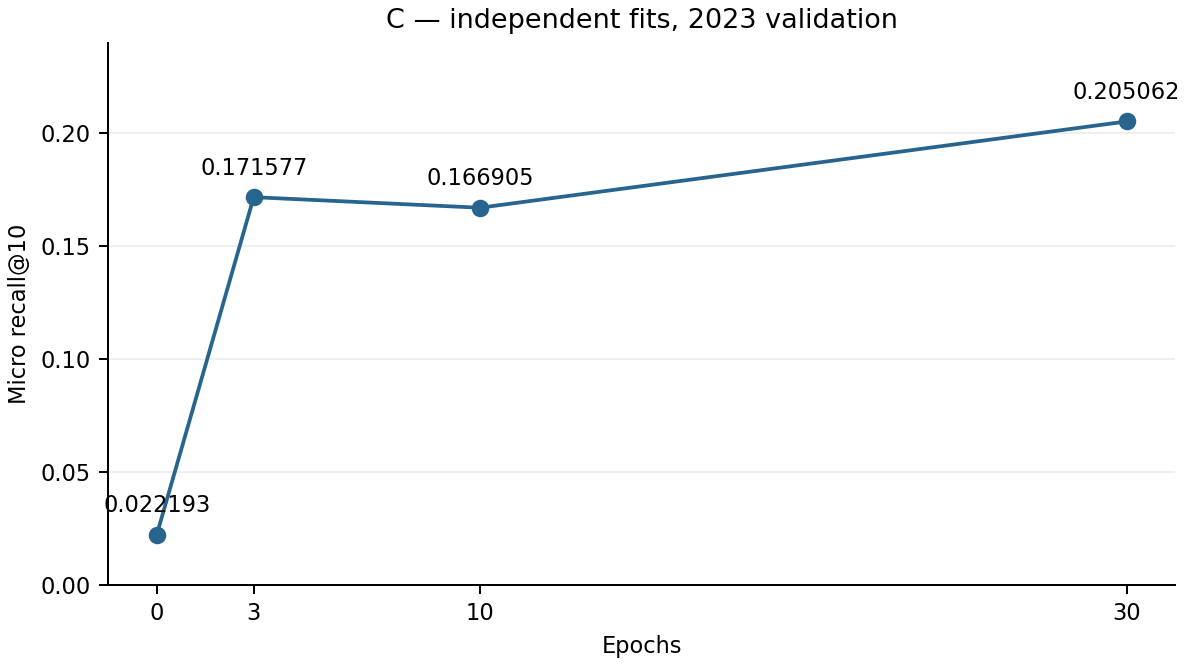
\includegraphics[width=\linewidth]{figures/maude_duration_RC2_en.png}
\caption{C: validation micro recall@10 by training duration. No training loss was observed for the zero-epoch fit.}
\label{fig:maude-duration-rc2}
\end{figure}

After selection, the chosen duration was fitted separately before 2024 and 2025, with rolling history between test quarters. On the 2024 test, micro recall@10 is $1,206/6,003=0.200899550225$; in 2025, $1,569/7,171=0.218797936132$. Summing hits and positive links across the two years gives $2,775/13,174=0.210642173979$, for 6,370 positive product--quarters and 2,975,156 candidate pairs. This pooled recall is not the arithmetic mean of the two annual recalls.

The historical benchmark test gave 0.172840443297 for three-epoch GraphSAGE and 0.192044936997 for neighbor frequency. These values remain unchanged. Prediction pairing, which is possible with retained historical outputs, must be distinguished from experimental control of duration. The absence of a new three-epoch fit in the C tests is not sufficient to make pairing impossible; conversely, matching keys and denominators do not demonstrate that duration alone explains a difference between training runs.

\subsection{Comparing the historical path with the C calculation}

The historical individual file records execution commit \src{ca0d64b2738c3f36637196cfb14d2fe4115a7c37}; \src{b010d5a49eae56837a920b2e30dece41c42c0c44} identifies the cited benchmark source state. Their role is distinct from C commit \src{4a22c2addc8203efd2b38a60c416270855c3bf3b}. Comparing sources between the historical execution and C shows no change to \src{evaluate.py}. In \src{models.py}, C adds loss/state callbacks and checkpoint reconstruction, and extracts the final representation calculation into a function.

\begin{table}[!htbp]\centering\footnotesize
\caption{Historical--C comparison of the mean-aggregation path. It describes code and retained evidence, not a new historical execution on health data.}
\begin{tabularx}{\linewidth}{@{}p{34mm}X@{}}
\toprule
Element & Comparison finding\\
\midrule
Initialization and neighborhood & Sorted node orders, sinusoidal vectors with salts 11/17, initial identity/0.25 transformations, and deterministic sampling of eight neighbors are unchanged.\\
Triplets and optimization & Product/positive order, epoch-dependent hashing, exclusion of positive neighbors, BPR coefficient, gradients, and regularized updates are unchanged; C adds counters and pre-update loss.\\
Representation and score & Same one-hop mean, $\tanh$, dot product, and zero fallback; extraction of the final calculation and raw-state export, without changing these operations.\\
Evaluation & Evaluation source unchanged; the new runner reads prepared snapshots, fits at annual origins, holds representations fixed during the year, and updates history after each quarter.\\
Evidence and limit & Retained preflight: 364 identical three-epoch scores on three non-empty fixtures, plus an empty case and checkpoint reconstruction. This non-health check does not prove equivalence of all possible executions.\\
\bottomrule
\end{tabularx}
\end{table}

Preflight reports and their fingerprints remain in \src{data/post_rc1/C_preflight.json}. Prepared snapshots do not expose every field of the historical \src{DataBundle}; this comparison concerns the graph-based GraphSAGE path, not all tabular methods. No historical model is retrained for this source verification. It supports interpreting C as configuration sensitivity, without turning selection on previously examined periods into a confirmatory experiment or a general causal effect of duration.

\subsection{GraphSAGE30--neighbors: paired comparison and conditional CI}

After this additional analysis was authorized on 3 October 2026, the protocol was fixed before the new calculation: 2024Q1--2025Q4 test, micro recall at ten, GraphSAGE30-minus-neighbors difference, 1,000 product draws with replacement, and seed 20261003. The selected model and historical results were already known; this calculation lock is therefore neither an external preregistration nor a correction for selection. No model is trained or scored.

Keys (product, quarter), support, and positive-problem sets agree across 6,370 observations, 13,174 positive links, and 2,026 products. C's complete candidate lists are checked against lists reconstructed from prepared snapshots and the unchanged historical rule; they total 2,975,156 pairs. The historical export does not retain its complete lists: it provides cardinalities and sampled positive/non-positive predictions. Agreement of reconstructed lists with C and of cardinalities/positives with the historical export is therefore established, not byte-for-byte identity of two complete exports. Any discrepancy would have stopped the analysis; no observation is removed through an opportunistic intersection.

Historical hits are read from \src{entity_metrics}, and C hits from retained ranks/labels, without recalculating scores. GraphSAGE30 retrieves 2,775 links and neighbors 2,530, on the same denominator of 13,174. The difference is $+0.018597236982$ and the conditional 95\,\% CI is $[+0.011975077183;+0.025570110820]$. Each draw keeps every quarter of a product together and recalculates the ratio of sums; this is neither a mean of product recalls nor independent resampling of quarters. The 2.5 and 97.5\,\% quantiles use linear interpolation; all 1,000 draws are defined.

The interval is conditional on the observed predictions and population. It covers neither validation selection, training variability, all network dependence between products, nor transfer to another population. It is neither independent confirmation nor a causal duration effect. It applies neither to historical three-epoch GraphSAGE nor to D1.

Pinned inputs, the protocol, contribution CSV, and draws are under \src{data/post_rc1/paired_*}; the source comparison is described in \src{verification/rc2_paired/code_bridge.json}. The completed calculation takes 7.969 s, with peak RSS of 488,841,216 bytes, below the 900 s / 512 MiB ceilings. A first attempt stopped before the draws: an address-space limit had been confused with the RSS ceiling. This mistakenly added restriction was removed without changing the RSS/time/output ceilings or statistical protocol; the record is retained in \src{verification/rc2_paired/attempt_1_failure.json}.

\paragraph{Original calculation in the repository, with retained outputs.}
\begin{Verbatim}[fontsize=\footnotesize]
python scripts/analyze_maude_paired_comparison.py \
  --protocol results/maude_paired_protocol_20261003.json \
  --output-dir NEW/maude_paired
\end{Verbatim}

\paragraph{Compact replay from the package root, without original inputs.}
\begin{Verbatim}[fontsize=\footnotesize]
PYTHONPATH=vendor/post_rc1 python \
  scripts/analyze_maude_paired_comparison.py \
  --protocol data/post_rc1/paired_protocol.json \
  --replay-contributions data/post_rc1/paired_contributions.csv \
  --output-dir NEW/maude_paired_replay
\end{Verbatim}
Use a new destination and an environment with NumPy (original calculation: Python 3.13.5, NumPy 2.3.5). Compact replay reproduces the contrast and draws but does not recheck original candidate identities. C/D1 checkpoints are included separately; their earlier audits are not rerun for this CI.


\subsection{D1: secondary neighborhood-removal diagnostic under fixed settings}

D1 compares C's 30-epoch \emph{mean} model, reused without refitting, with one new 30-epoch \emph{none} model. The shared duration comes from C and the fixed D1 protocol; no duration grid or duration tuning was conducted in D1. The same periods and evaluation rules are used for both variants: candidate identifiers, labels, support counts, hashed negatives, and ranking conventions agree. Both models retain trainable node-identity vectors. The \emph{none} model computes $h=\tanh(W_{\mathrm{self}}x)$ from the node's own vector only; it does not aggregate neighbors and is not a GNN.

Absence of message passing does not mean absence of relational information: \emph{none}'s identity vectors are learned from the same historical edges and BPR. D1 compares two ways of calculating and learning representations. Duration was selected for \emph{mean}, then imposed on \emph{none}; no control-specific tuning established its ability to optimize this task effectively.

The \emph{mean} variant has 128 active shared-transformation scalars, compared with 64 for \emph{none}; the number of node-vector scalars is the same in each pair of fits. This 64-parameter difference must be declared, but it does not demonstrate that capacity explains the gap. The imposed duration and the control's nearly flat loss are also essential to interpreting this diagnostic. The contrast does not isolate a causal aggregation effect at equal capacity.

D1 was locked at 20:53:30.842192 UTC using validation, before its first D1-specific tests. However, the C test results for \emph{mean} were already available at that lock, and the test periods had been consulted earlier. Thus, the ordering of the D1 lock and its tests does not make this an independent confirmation.

\begin{table}[!htbp]\centering\scriptsize\setlength{\tabcolsep}{2.5pt}
\caption{D1: micro recall@10 on cohorts with at least one positive link, at historical support $\geq1$. Mean30 is retained from C; none30 was newly fitted in D1. Hits are shown in parentheses. No interval is attached to the contrast.}
\label{tab:aggregation-rc2}
\begin{tabularx}{\linewidth}{@{}XrXXr@{}}
\toprule
Cohort & Positive links & Mean30 R@10 (hits) & None30 R@10 (hits) & Mean $-$ none\\
\midrule
Validation 2023 & 7,705 & 0.205061648 (1,580) & 0.031148605 (240) & $+0.173913043$\\
Test 2024 & 6,003 & 0.200899550 (1,206) & 0.036481759 (219) & $+0.164417791$\\
Test 2025 & 7,171 & 0.218797936 (1,569) & 0.034862641 (250) & $+0.183935295$\\
Pooled test 2024--2025 & 13,174 & 0.210642174 (2,775) & 0.035600425 (469) & $+0.175041749$\\
\bottomrule
\end{tabularx}
\end{table}

On the pooled test, mean30 obtains $2,775/13,174=0.210642173979$ and none30 $469/13,174=0.035600425080$; the signed descriptive mean30--none30 difference is $+0.175041748899$. No confidence interval or statistical test is attached to this difference. The figure also shows the annual contrasts and recorded losses.

\begin{figure}[!htbp]\centering
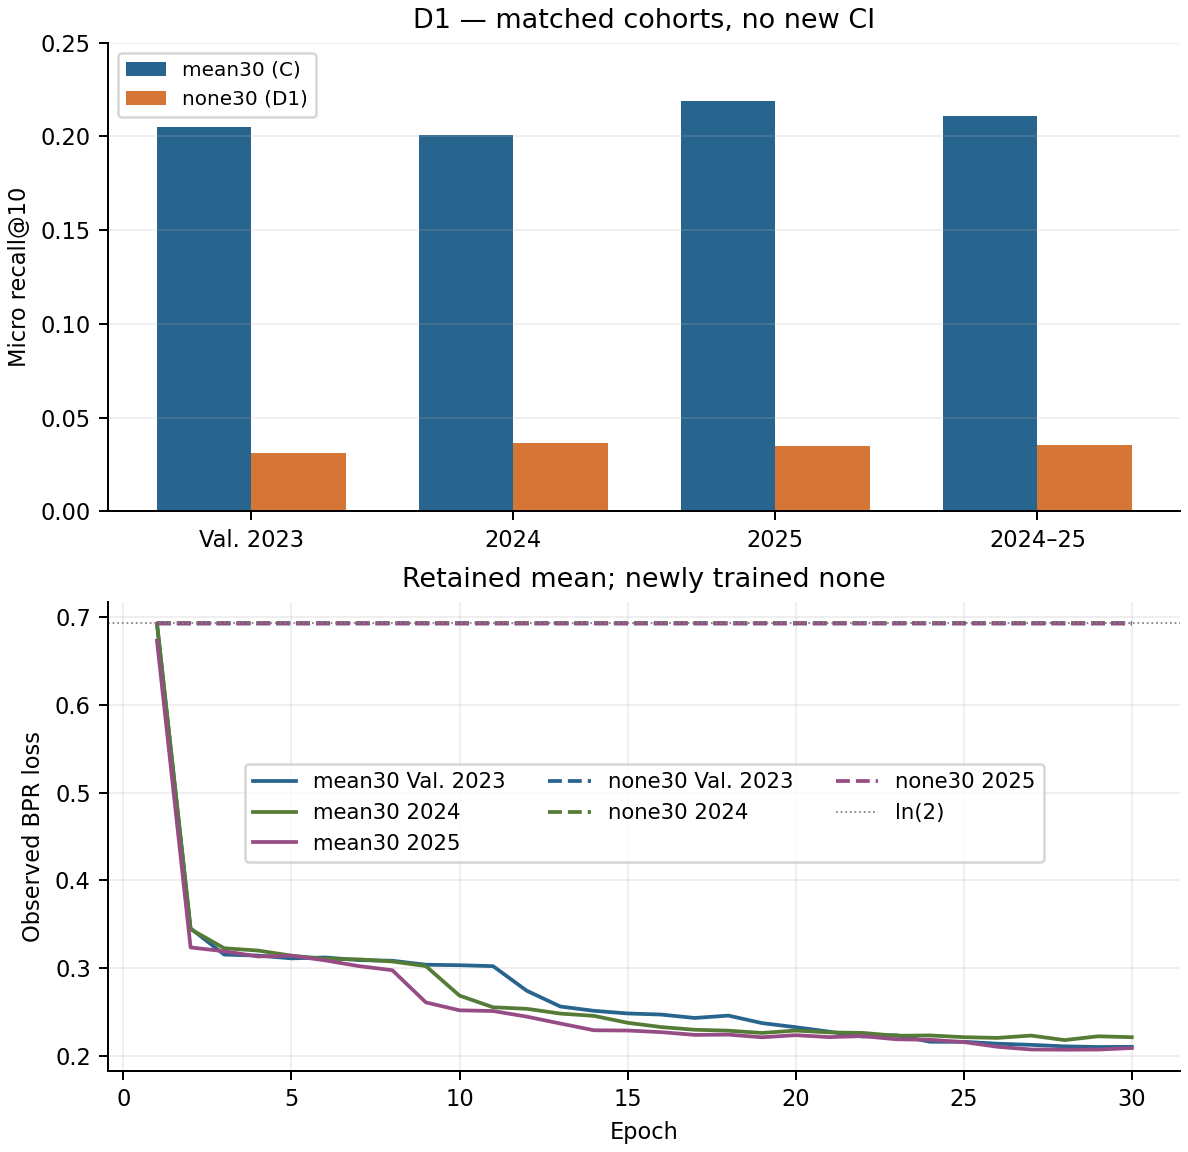
\includegraphics[width=\linewidth]{figures/maude_aggregation_RC2_en.png}
\caption{D1: micro recalls@10 in the upper panel; observed losses in the lower panel. Mean30 is reused from C; only the none30 fits are new in D1. Pooled recall combines the two test years and is not an additional distinct cohort.}
\label{fig:maude-aggregation-rc2}
\end{figure}

The three none30 fits comprise 90 observed epochs, 6,756,720 steps, and no skipped positives. The exported data loss, the pre-update mean of $\operatorname{softplus}(-\text{margin})$ excluding regularization, remains close to $\ln(2)$ with no observed decrease (about 0.693132--0.693145 at the first epoch and 0.693147 at the thirtieth). This finding is more informative about the control's scope than recall-bar height alone: it does not establish effective learning under the retained parameters. However, it identifies neither a bug, representation collapse, too few epochs, nor another cause of failure. D1 remains a sensitivity diagnostic for neighborhood removal under fixed settings, not a demonstration of the causal benefit of aggregation.

\subsection{Audits, costs, and scope of verification}

C and D1 audits concern the new fits and do not replace the historical B1/B2 reconstruction in S10. The C audit reconstructs scores from six raw checkpoints and checks 9,449,508 predictions, 24 fit-quarters, and 20,302 candidate lists; no discrepancy is detected, with an absolute tolerance of $10^{-12}$ for floating-point values. The report is retained under \src{verification/post_rc1/C_numeric_audit.json}, with the manifest \src{data/post_rc1/C_manifest.json}. The earlier B1/B2 reconstructions recovered training inputs and node inventories without inspecting historical checkpoints.

The D1 audit reconstructs none30 scores from three raw checkpoints and pairs them with C's retained mean30 outputs. It checks 4,593,744 new scores, 9,853 candidate lists per variant, 12 quarters, and 51,260,776 numerical checks; no discrepancy is detected at the absolute tolerance of $10^{-12}$. The 9,187,488 candidate identifiers are the sum of the two exports, or 4,593,744 pairs on each side. The D1 audit took 58.547 s. Its final memory readings diverge: $118,292,480$ bytes for \texttt{VmHWM} and \texttt{VmRSS}, versus $571,580,416$ bytes for \texttt{ru\_maxrss}. In the absence of startup readings, it is not possible to certify that the entire audit stayed below 512 MiB or to attribute the discrepancy with certainty to the process or launcher. An independent telemetry probe shows that a different scope after \texttt{exec} can explain the discrepancy, without establishing the exact source of this audit measurement. Both values remain recorded in \src{data/post_rc1/post_rc1_metrics.json}.

For training phases, the limits were 900 s, 512 MiB aggregate RSS, and 512 MiB of output per phase, with one worker and a single-threaded environment; each reported C and D1 phase finished within these limits, without retries. C totaled 1,167.908 s across its phases (maximum aggregate RSS peak 249,405,440 bytes); this sum across multiple phases was not subject to a global 900-s limit. D1 totaled 416.144 s (maximum aggregate RSS peak 303,284,224 bytes). Mean30 measurements are from C and were reused; they are not new fitting costs incurred by D1. These costs do not establish equal CPU budgets between variants or runs.

These checks establish numerical consistency of RC2 outputs with the prepared snapshots, checkpoints, and audited logs. They do not verify historical public availability of every field, undo prior exposure to the periods, provide independent confirmation or clinical benefit, or justify causal or general claims about graphs.

\section{Open items and editorial preparation}
\label{supp:open}
RC2 incorporates the exploratory MAUDE C/D1 analyses in S11 while preserving historical tables and intervals. The R6 review and response remain historical material, not an assessment or approval of RC2. Technical package checks are recorded in \src{verification/rc2}; they do not replace the authors' scientific and bibliographic approval. The manuscript has not been submitted or accepted.

The earlier R3 source corrected the RelBench v2 venue to \emph{3rd DATA-FM Workshop at ICLR 2026}, matching the venue printed on the article's first page rather than describing it as a main-conference paper\cite{gu2026relbench}. That earlier revision also added a precise synthetic-control reference and harmonized provenance notes; no new exhaustive literature search is claimed for RC2.

The target journal and its length, language, anonymization, and formatting requirements remain to be selected. The inherited FAIA name denotes a book and proceedings series, not a journal choice. \src{submission_ios_fr.tex} and \src{submission_ios_en.tex} are IOS-class entrypoints; they have not been compiled or validated here for a final venue. Delivered PDFs use the reading layout.

Finally, author names, affiliations, corresponding author, contributions, funding, competing interests, ethics position, data-use conditions, and AI-assistance disclosure require author approval. Missing fields must not be replaced by “none” or an assumed exemption. Any retained proposed reviewer-response items are historical unsent working materials, not a signed attestation, an RC2 response, or a completed submission.

\bibliographystyle{unsrtnat}
\bibliography{references}
\end{document}
